% !TeX root = ../thesis.tex
\chapter{Appendices to Chapter 7 (PASTURE analysis)}
\label{sec:app:application}

%====================================
\section{Within-sample diversity across remaining cohort variables}
\label{sec:app:7app:alpha_remaining}
%====================================

The following figures show within-sample diversity estimates for the cohort variables that were not selected as the main grouping variable in Chapter~\ref{ch:application}. Richness was estimated using \texttt{breakaway}, whereas Shannon diversity and the Gini--Simpson index were estimated using \texttt{DivNet}. For each variable and diversity measure, an overall Kruskal--Wallis test was performed first using the standard asymptotic approximation. If the overall test was significant and the variable had more than two groups, pairwise Wilcoxon rank-sum tests were carried out for all group combinations. For variables with two groups, the Wilcoxon rank-sum test corresponds to the group comparison shown in the figure. Reported p-values are asymptotic p-values and are displayed only for significant comparisons.

%------------------------------------
% alpha diversity: country
%------------------------------------
\begin{figure}[H]
\centering
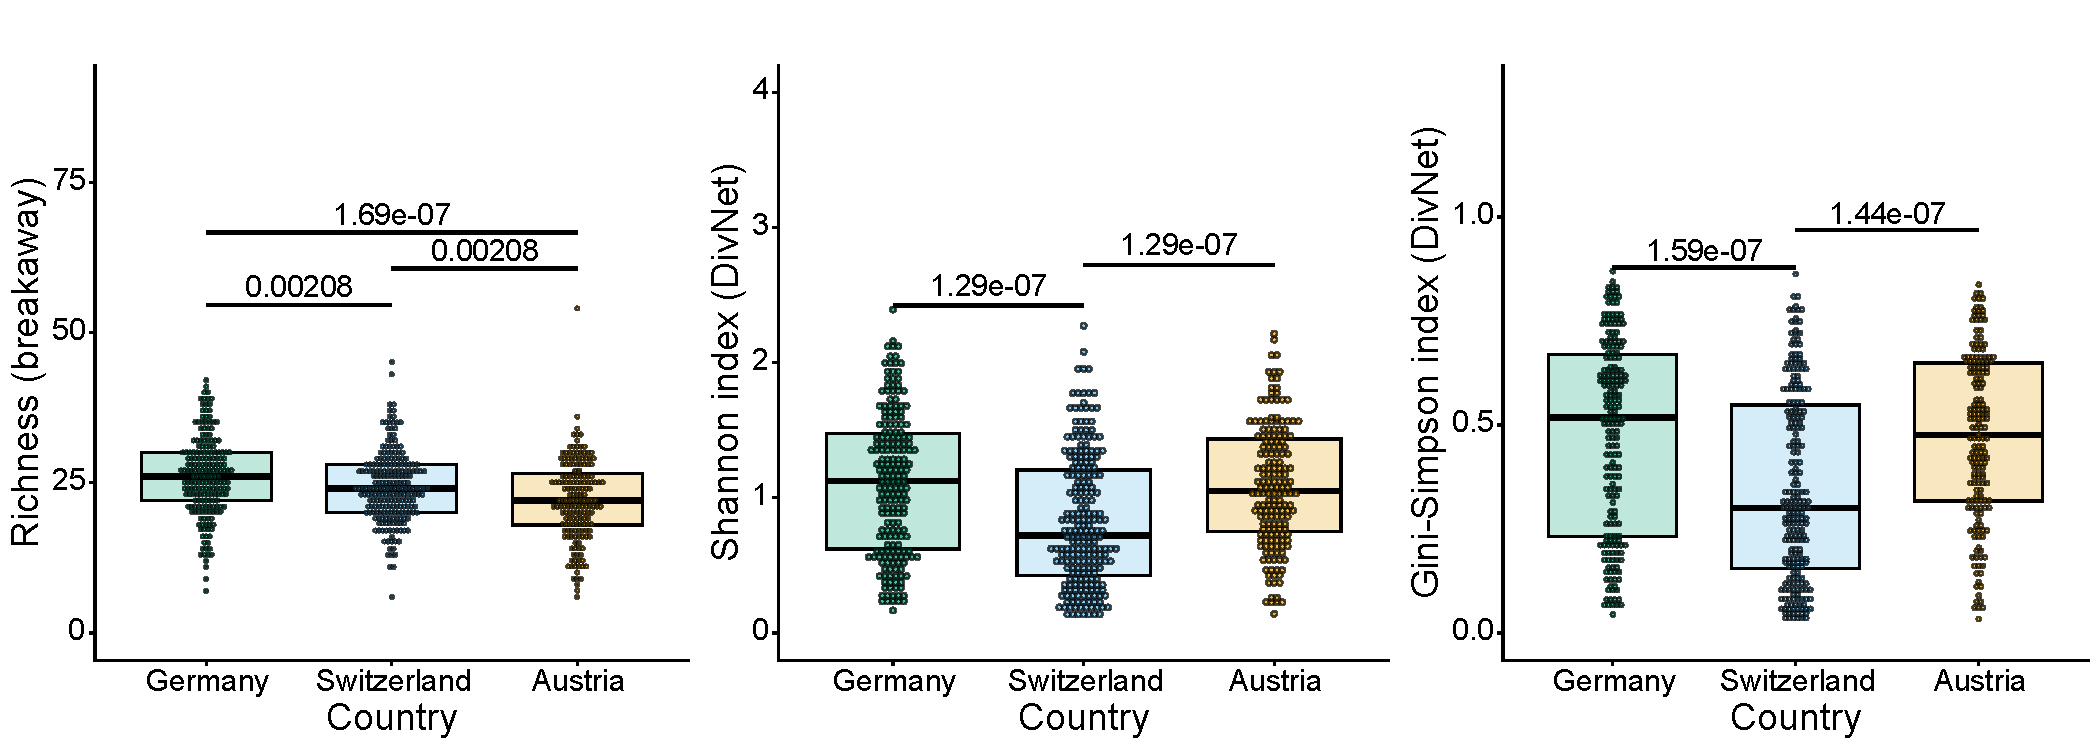
\includegraphics[width=\textwidth]{../ch07_application/figures/03_alpha_diversity/Country_2m-1.pdf}
\caption{\textbf{Within-sample diversity by country.} Sample-wise estimates of richness, Shannon diversity, and Gini--Simpson diversity stratified by country. Sample sizes are 173 for Austria, 197 for Germany, and 222 for Switzerland.}
\label{fig:app:7app:alpha_div_country}
\end{figure}

%------------------------------------
% alpha diversity: sex
%------------------------------------
\begin{figure}[H]
\centering
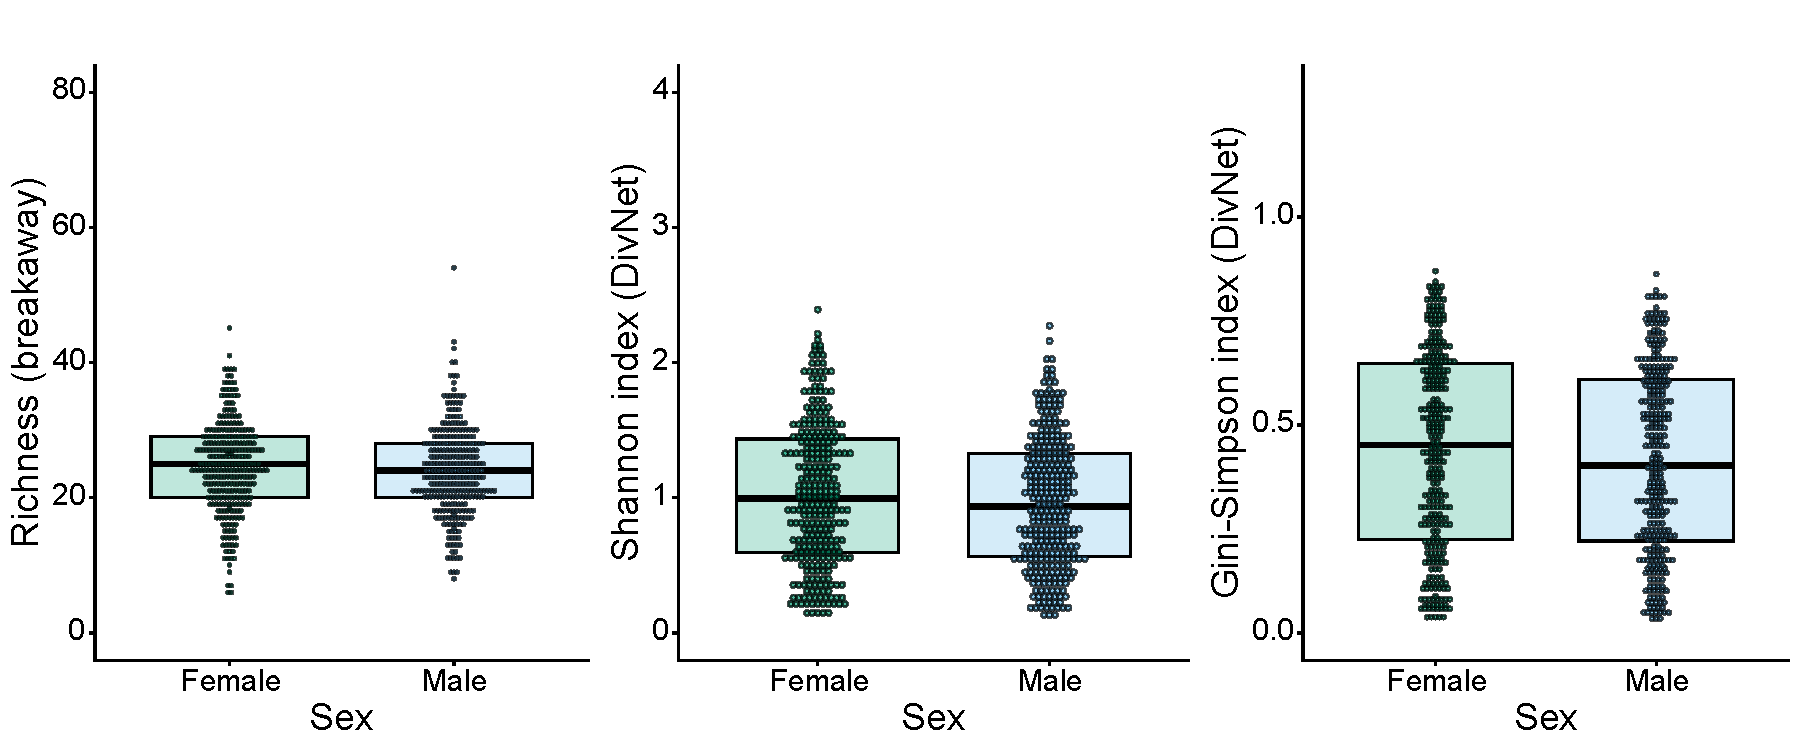
\includegraphics[width=\textwidth]{../ch07_application/figures/03_alpha_diversity/sex_2m-1.pdf}
\caption{\textbf{Within-sample diversity by sex.} Sample-wise estimates of richness, Shannon diversity, and Gini--Simpson diversity stratified by child sex. Sample sizes are 294 for female and 298 for male children.}
\label{fig:app:7app:alpha_div_sex}
\end{figure}

%------------------------------------
% alpha diversity: delivery mode
%------------------------------------
\begin{figure}[H]
\centering
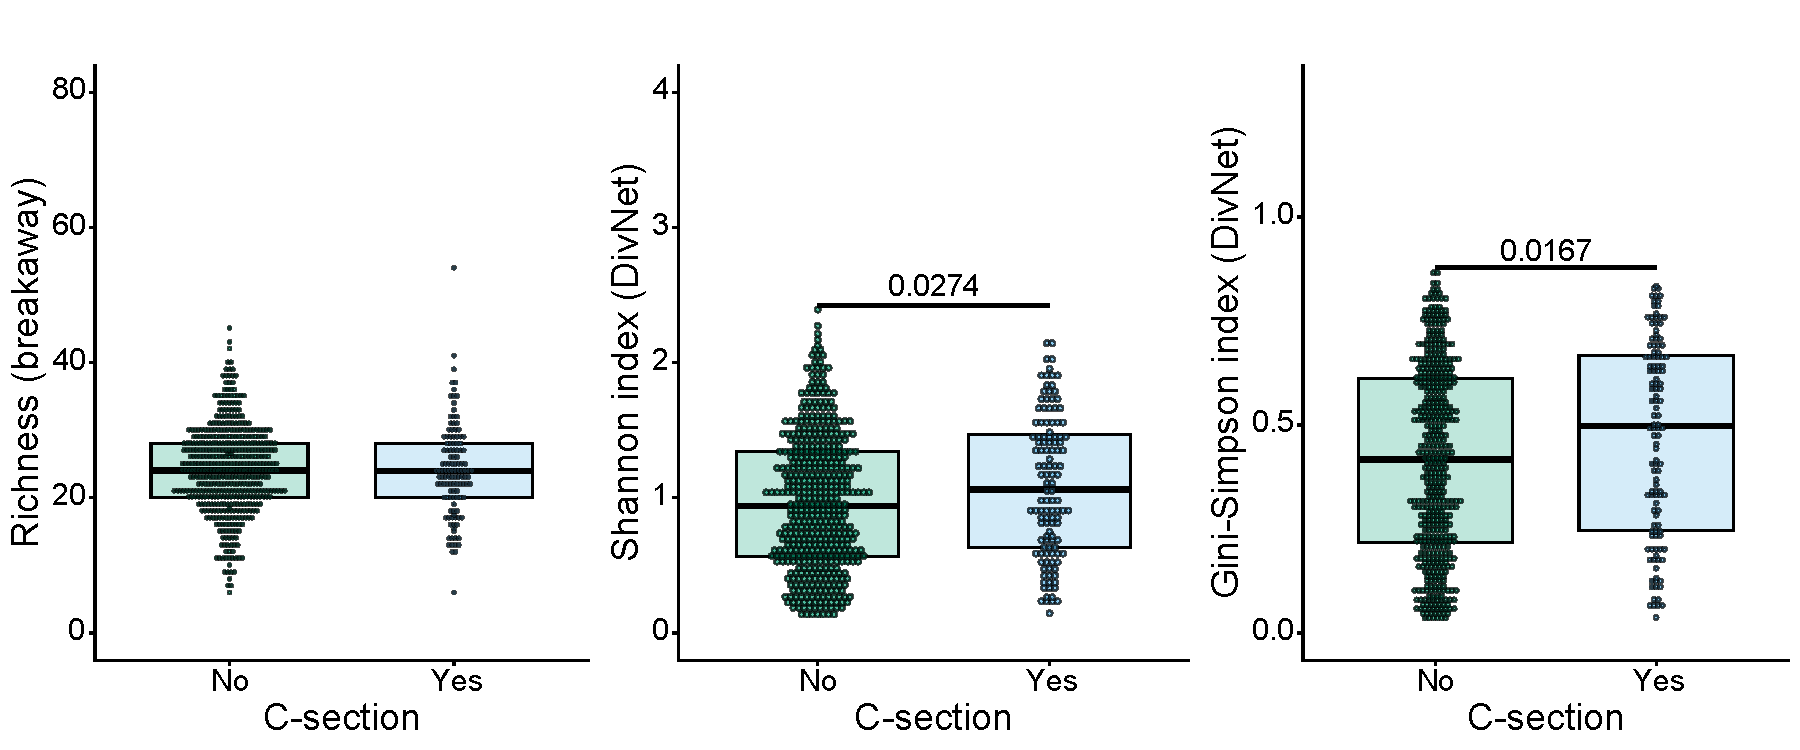
\includegraphics[width=\textwidth]{../ch07_application/figures/03_alpha_diversity/cesarean_2m-1.pdf}
\caption{\textbf{Within-sample diversity by delivery mode.} Sample-wise estimates of richness, Shannon diversity, and Gini--Simpson diversity stratified by delivery mode. Sample sizes are 468 for vaginal delivery and 121 for delivery by cesarean section.}
\label{fig:app:7app:alpha_div_csection}
\end{figure}

%------------------------------------
% alpha diversity: breastfeeding duration
%------------------------------------
\begin{figure}[H]
\centering
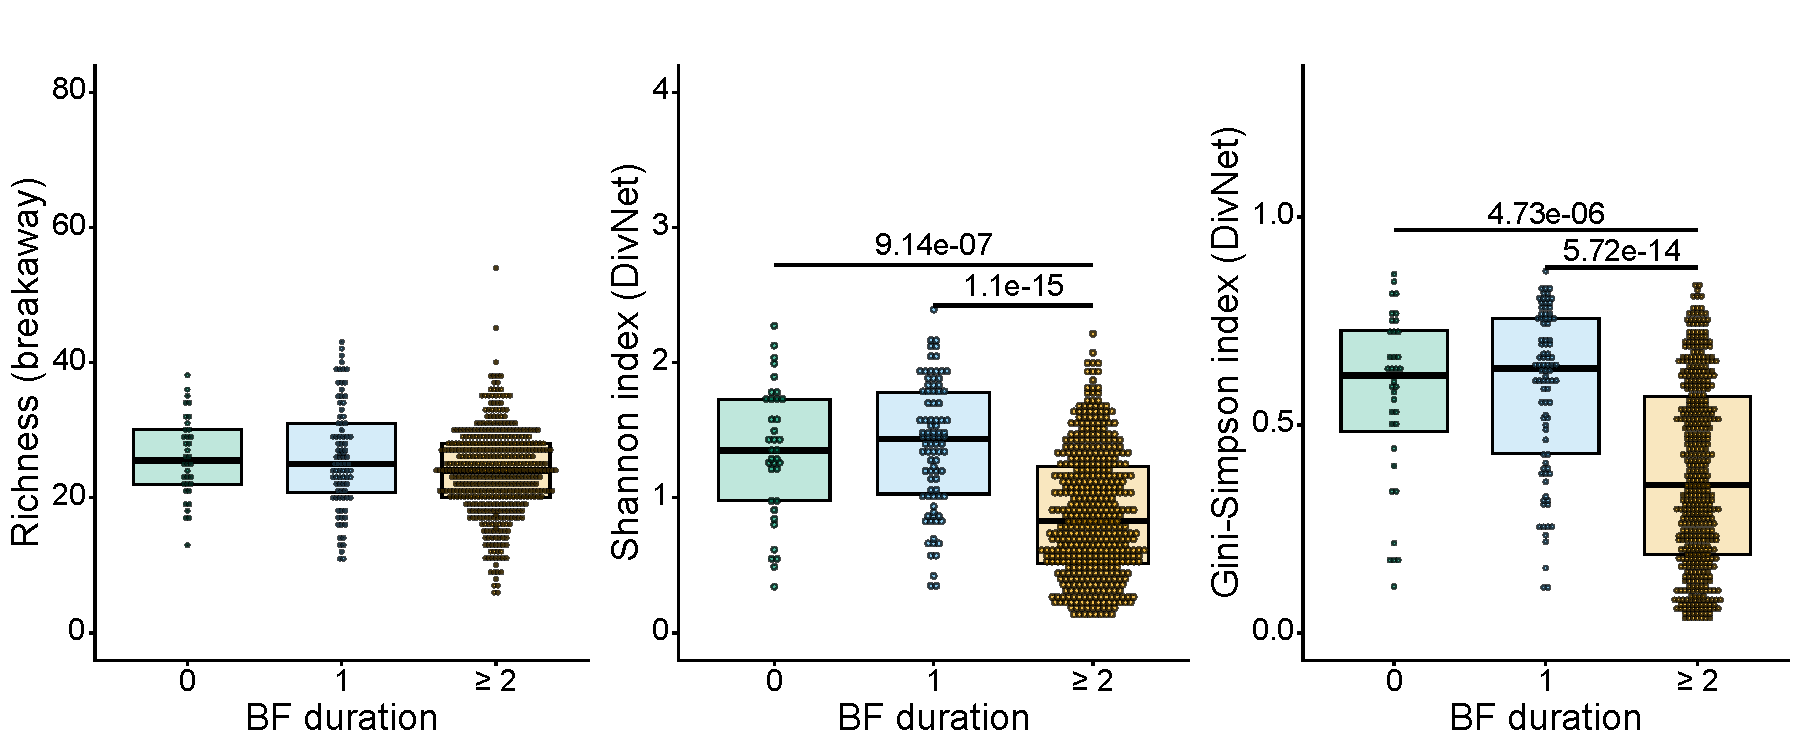
\includegraphics[width=\textwidth]{../ch07_application/figures/03_alpha_diversity/breastfeed_2m-1.pdf}
\caption{\textbf{Within-sample diversity by breastfeeding duration.} Sample-wise estimates of richness, Shannon diversity, and Gini--Simpson diversity stratified by total breastfeeding duration. Sample sizes are 36 for no breastfeeding, 88 for one month of breastfeeding, and 456 for at least two months of breastfeeding.}
\label{fig:app:7app:alpha_div_bf_duration}
\end{figure}

%------------------------------------
% alpha diversity: prenatal smoking
%------------------------------------
\begin{figure}[H]
\centering
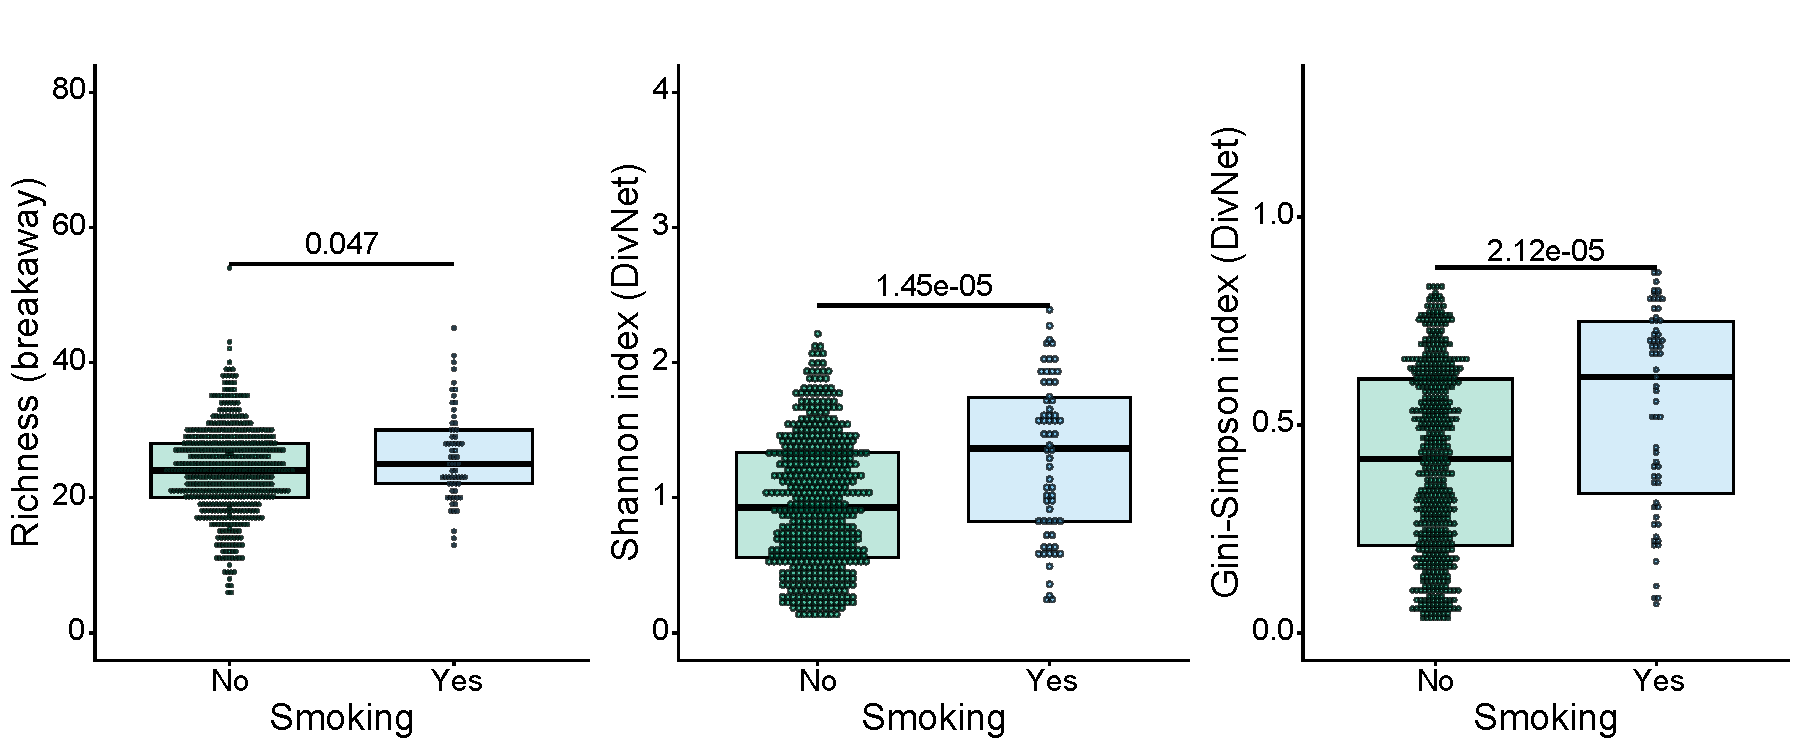
\includegraphics[width=\textwidth]{../ch07_application/figures/03_alpha_diversity/pregsmoke_2m-1.pdf}
\caption{\textbf{Within-sample diversity by prenatal smoking.} Sample-wise estimates of richness, Shannon diversity, and Gini--Simpson diversity stratified by maternal smoking during pregnancy. Sample sizes are 529 for no prenatal smoking and 63 for prenatal smoking.}
\label{fig:app:7app:alpha_div_smoking}
\end{figure}

%------------------------------------
% alpha diversity: number of older siblings
%------------------------------------
\begin{figure}[H]
\centering
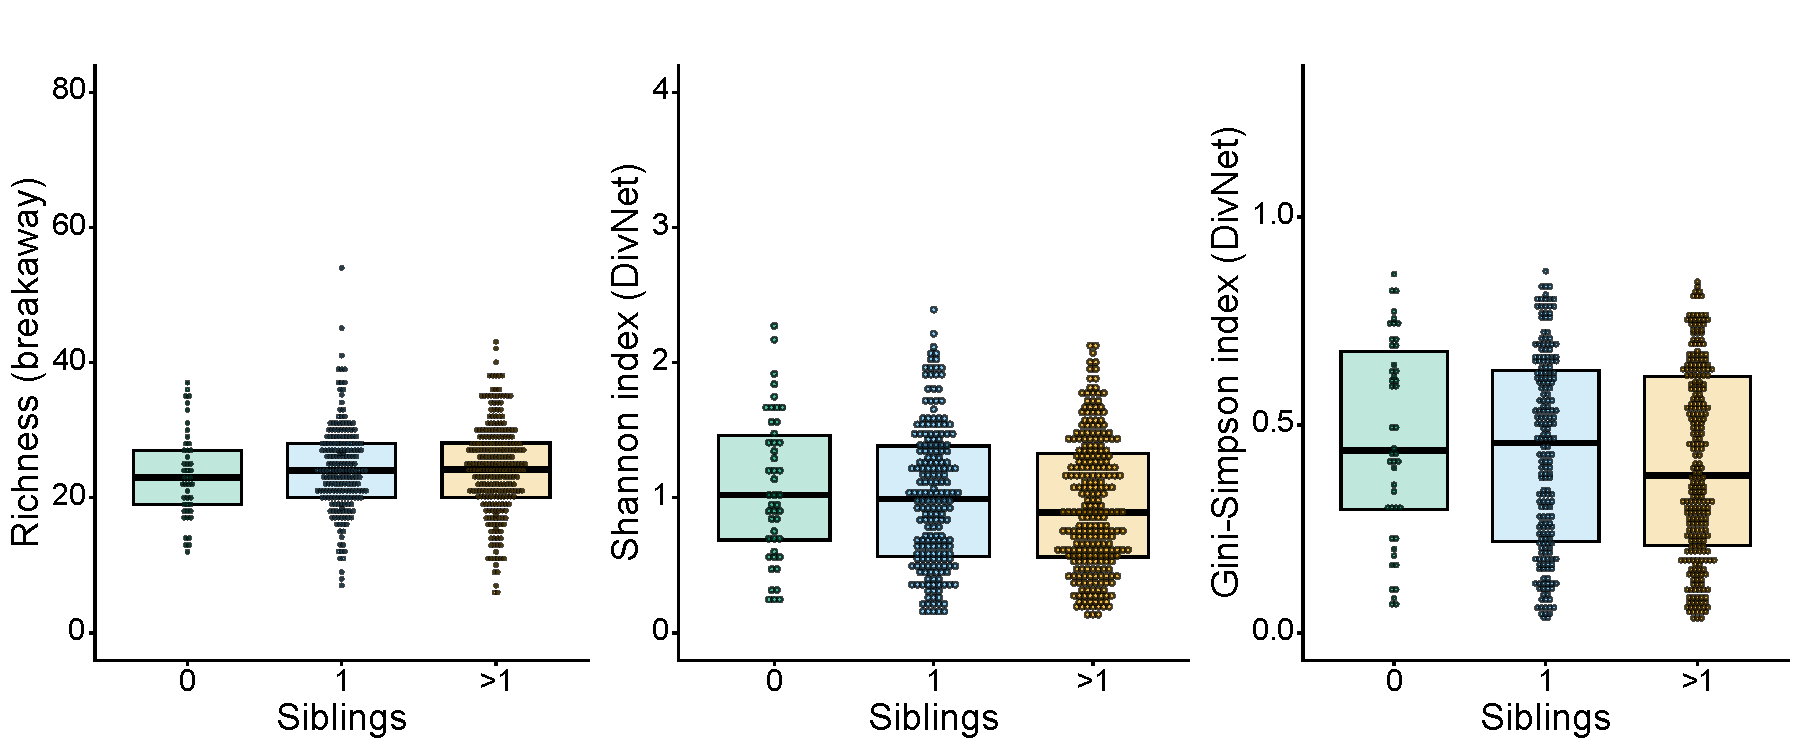
\includegraphics[width=\textwidth]{../ch07_application/figures/03_alpha_diversity/sibsnumb_2m-1.pdf}
\caption{\textbf{Within-sample diversity by number of older siblings.} Sample-wise estimates of richness, Shannon diversity, and Gini--Simpson diversity stratified by the number of older siblings. Sample sizes are 46 for no older siblings, 200 for one older sibling, and 257 for more than one older sibling.}
\label{fig:app:7app:alpha_div_siblings}
\end{figure}

%====================================
\section{Compositional equivalence}
\label{sec:app:7app:comp_equivalence}
%====================================

\begin{figure}[H]
\centering
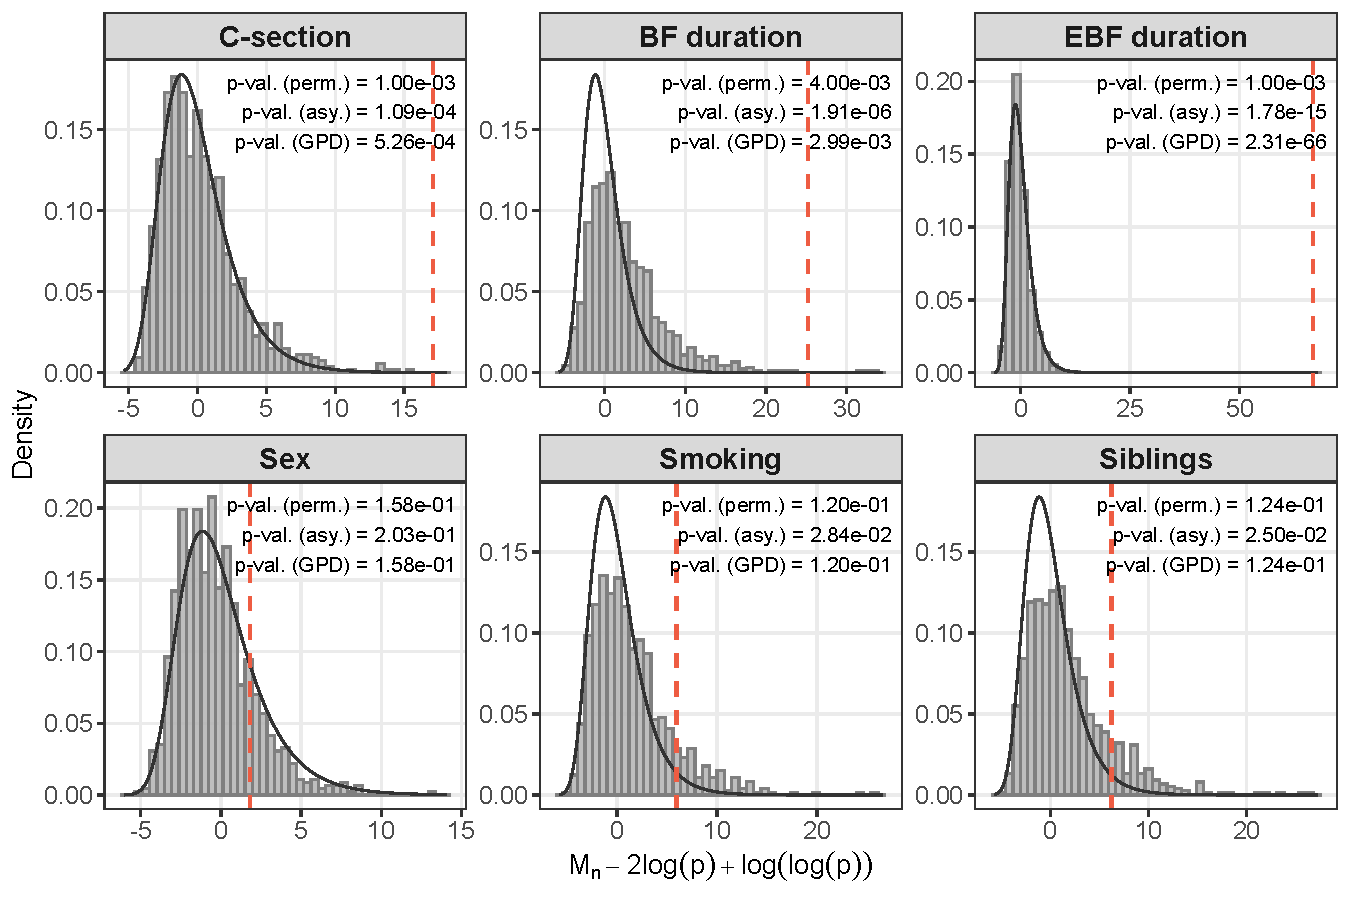
\includegraphics[width=\textwidth]{../ch07_application/figures/06_comp_equivalence/comp_equivalence_gumbel_comparison_plot-1.pdf}
\caption{\textbf{Comparison of permutation-based and asymptotic null distributions for compositional equivalence.}
For each selected two-group contrast, the gray histogram shows the permutation distribution of the centered statistic $M_n - 2\log(p) + \log\log(p)$, where $M_n$ is the maximum standardized squared CLR mean difference and $p$ is the number of tested CLR coordinates. The gray curve shows the asymptotic Gumbel density proposed by \citet{cao2018twosample}, and the red dashed line marks the observed centered statistic. Annotated p-values show the empirical permutation p-value, the asymptotic Gumbel p-value, and the GPD-refined permutation p-value obtained with \texttt{permApprox}. The comparison illustrates that the asymptotic Gumbel approximation does not uniformly match the permutation null distributions for the PASTURE contrasts.}
\label{fig:app:7app:comp_equivalence_gumbel_comparison}
\end{figure}

%====================================
\section{Differential abundance analysis}
\label{sec:app:7app:diff_abundance}
%====================================

\begin{table}[H]
\centering
\caption{textbf{Adjusted p-values for selected differential abundance analyses.} The table shows genera with Benjamini--Hochberg-adjusted p-values below $\alpha=0.01$ in at least one selected differential abundance analysis. Rows are ordered by increasing adjusted \texttt{permApprox} p-values. The DACOMP statistic $T$ is the observed test statistic used for the permutation test. DACOMP columns show adjusted empirical permutation p-values with the indicated number of permutations, and the \texttt{permApprox} column shows adjusted p-values obtained from constrained GPD tail approximation based on the $1000$-permutation DACOMP run.}
\label{tab:app:7app:diff_abundance_adj_pvalues}\
\vspace{0.5em}
\small
\begin{tabular}{lrlll}
\toprule
Taxon & $T$ & DACOMP ($10^3$) & DACOMP ($10^7$) & \texttt{permApprox} \\
\midrule
\emph{Enterococcus} & $75.64$ & 6.77e-03$^{**}$ & 9.80e-07$^{***}$ & 2.34e-94$^{***}$ \\
\emph{Lactococcus} & $28.84$ & 6.77e-03$^{**}$ & 9.80e-07$^{***}$ & 9.85e-25$^{***}$ \\
\emph{Intestinibacter} & $48.86$ & 6.77e-03$^{**}$ & 9.80e-07$^{***}$ & 3.10e-14$^{***}$ \\
\emph{Streptococcus} & $16.66$ & 6.77e-03$^{**}$ & 1.02e-04$^{***}$ & 1.18e-09$^{***}$ \\
\emph{[Clostridium] innocuum group} & $32.17$ & 6.77e-03$^{**}$ & 1.09e-04$^{***}$ & 3.95e-07$^{***}$ \\
\emph{[Ruminococcus] gnavus group} & $32.23$ & 6.77e-03$^{**}$ & 9.80e-07$^{***}$ & 4.97e-07$^{***}$ \\
\emph{Bifidobacterium} & $36.76$ & 6.77e-03$^{**}$ & 9.80e-07$^{***}$ & 2.50e-05$^{***}$ \\
\emph{Blautia} & $20.75$ & 6.77e-03$^{**}$ & 1.29e-03$^{**}$ & 9.17e-05$^{***}$ \\
\emph{Terrisporobacter} & $20.92$ & 6.77e-03$^{**}$ & 1.68e-03$^{**}$ & 1.96e-03$^{**}$ \\
\addlinespace
\emph{uncultured18} & $13.31$ & 1.28e-02$^{*}$ & 2.97e-03$^{**}$ & 5.06e-02 \\
\emph{Clostridium sensu stricto 1} & $8.04$ & 3.40e-02$^{*}$ & 3.53e-03$^{**}$ & 5.48e-02 \\
\emph{Collinsella} & $6.42$ & 4.14e-02$^{*}$ & 2.97e-03$^{**}$ & 7.09e-02 \\
\emph{[Ruminococcus] torque group} & $8.52$ & 1.82e-02$^{*}$ & 2.97e-03$^{**}$ & 9.64e-02 \\
\emph{Sellimonas} & $3.58$ & 1.53e-01 & 7.76e-03$^{**}$ & 1.62e-01 \\
\emph{Tyzzerella} & $4.47$ & 1.25e-01 & 6.80e-04$^{***}$ & 1.75e-01 \\
\bottomrule
\end{tabular}

\begin{minipage}{0.98\textwidth}
\small
Significance codes refer to adjusted p-values: $^{*} q < 0.05$, $^{**} q < 0.01$, and $^{***} q < 0.001$.
\end{minipage}
\end{table}

%====================================
\section{Differential distribution analysis}
\label{sec:app:7app:diff_distribution}
%====================================

\begin{table}[H]
\centering
\caption{\textbf{Adjusted p-values for selected differential distribution analyses.} The table shows Benjamini--Hochberg-adjusted p-values for genera with an adjusted p-value below $\alpha=0.01$ in at least one panel of Figure~\ref{fig:7app:dd:volcano}. The columns correspond to the non-zero Wasserstein component, the zero-prevalence component, the combined two-stage result, and the one-stage complete-CLR analysis. The non-zero, combined, and one-stage results use constrained \texttt{permApprox} refinement.}
\label{tab:app:7app:diff_distribution_pvalues_all_approaches}
\vspace{0.5em}
\small
\begin{tabular}{lllll}
\toprule
Taxon & Non-zero & Zero prev. & Combined & One-stage \\
\midrule
\emph{Intestinibacter} & 1.35e-10$^{***}$ & 1.19e-02$^{*}$ & 3.50e-12$^{***}$ & 3.39e-44$^{***}$ \\
\emph{Enterococcus} & 7.00e-07$^{***}$ & 8.38e-02 & 1.70e-07$^{***}$ & 8.05e-28$^{***}$ \\
\emph{Lactococcus} & 2.68e-04$^{***}$ & 9.40e-04$^{***}$ & 1.28e-07$^{***}$ & 1.40e-25$^{***}$ \\
\emph{[Ruminococcus]\_gnavugroup} & 2.01e-10$^{***}$ & 7.31e-01 & 3.11e-09$^{***}$ & 6.27e-15$^{***}$ \\
\emph{[Clostridium]\_innocuum\_group} & 5.75e-05$^{***}$ & 4.83e-01 & 1.79e-04$^{***}$ & 7.10e-10$^{***}$ \\
\addlinespace
\emph{Blautia} & 7.05e-09$^{***}$ & 7.79e-01 & 1.01e-07$^{***}$ & 8.08e-07$^{***}$ \\
\emph{Akkermansia} & 5.75e-05$^{***}$ & 1.44e-02$^{*}$ & 1.58e-06$^{***}$ & 1.86e-03$^{**}$ \\
\emph{Erysipelatoclostridium} & 1.59e-06$^{***}$ & 2.17e-01 & 1.84e-06$^{***}$ & 2.89e-03$^{**}$ \\
\emph{Bacteroides} & 2.52e-03$^{**}$ & 6.64e-02 & 2.51e-04$^{***}$ & 4.58e-06$^{***}$ \\
\emph{Streptococcus} & 1.45e-05$^{***}$ & 4.83e-01 & 5.25e-05$^{***}$ & 5.21e-06$^{***}$ \\
\addlinespace
\emph{[Ruminococcus]\_torquegroup} & 1.82e-05$^{***}$ & 4.83e-01 & 6.04e-05$^{***}$ & 2.19e-03$^{**}$ \\
\emph{Terrisporobacter} & 2.24e-02$^{*}$ & 2.71e-03$^{**}$ & 6.03e-05$^{***}$ & 3.11e-05$^{***}$ \\
\emph{Tyzzerella} & 5.75e-04$^{***}$ & 2.09e-01 & 4.32e-04$^{***}$ & 9.47e-05$^{***}$ \\
\emph{Leuconostoc} & 7.18e-01 & 1.59e-03$^{**}$ & 1.84e-03$^{**}$ & 1.37e-04$^{***}$ \\
\emph{Collinsella} & 1.25e-03$^{**}$ & 6.64e-02 & 1.52e-04$^{***}$ & 1.34e-03$^{**}$ \\
\addlinespace
\emph{Haemophilus} & 9.64e-01 & 1.33e-03$^{**}$ & 1.84e-03$^{**}$ & 4.05e-04$^{***}$ \\
\emph{Corynebacterium} & 5.52e-01 & 1.09e-02$^{*}$ & 9.43e-03$^{**}$ & 9.24e-04$^{***}$ \\
\emph{uncultured18} & 6.38e-02 & 6.98e-02 & 6.99e-03$^{**}$ & 2.39e-03$^{**}$ \\
\emph{Lactobacillus} & 7.02e-01 & 8.05e-03$^{**}$ & 9.43e-03$^{**}$ & 4.21e-03$^{**}$ \\
\emph{Epulopiscium} & 7.75e-01 & 2.60e-02$^{*}$ & 4.60e-02$^{*}$ & 5.13e-03$^{**}$ \\
\addlinespace
\emph{Coprobacillus} & -- & 8.38e-02 & 5.18e-02 & 5.49e-03$^{**}$ \\
\emph{Granulicatella} & 2.80e-01 & 6.98e-02 & 3.02e-02$^{*}$ & 5.49e-03$^{**}$ \\
\emph{Scardovia} & 5.55e-01 & 8.94e-02 & 1.04e-01 & 5.71e-03$^{**}$ \\
\emph{Clostridium\_sensu\_strict1} & 8.11e-03$^{**}$ & 3.10e-01 & 7.99e-03$^{**}$ & 1.03e-02$^{*}$ \\
\emph{Anaerostipes} & 8.15e-03$^{**}$ & 4.83e-01 & 1.45e-02$^{*}$ & 2.68e-01 \\
\bottomrule
\end{tabular}

\vspace{0.4em}
\begin{minipage}{0.95\textwidth}
\small
Significance codes refer to adjusted p-values: $^{*} q < 0.05$, $^{**} q < 0.01$, and $^{***} q < 0.001$.\\
The symbol ``--'' indicates that the corresponding statistic could not be computed.
\end{minipage}
\end{table}

%====================================
\section{Network analysis}
\label{sec:app:7app:net_analysis}
%====================================

\begin{figure}[H]
\centering
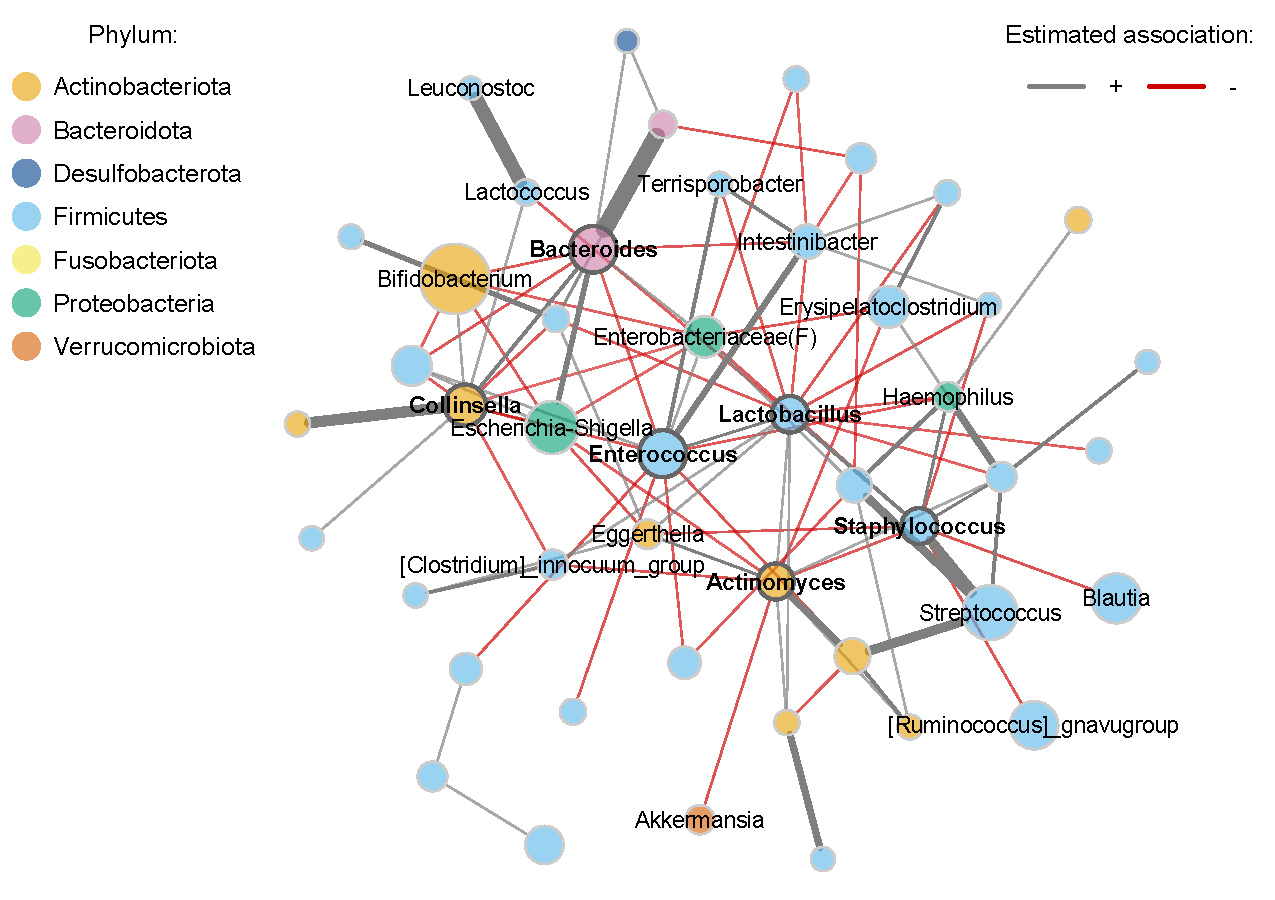
\includegraphics[width=\textwidth]{../ch07_application/figures/10_network_analysis/single_net_plot_slr_slrlay-1.pdf}
\caption{\textbf{SPIEC-EASI SLR association network with spring layout.} The network was estimated from the complete default data set using the SPIEC-EASI sparse-plus-low-rank (SLR) approach with the rank selected by the Bayesian information criterion, as described in Section~\ref{sec:7app:network:sensitivity}. Nodes represent genera and are colored according to phylum, while node sizes are proportional to the mean CLR coordinate across samples. Gray and red edges indicate positive and negative estimated conditional associations, respectively. Node positions were determined by a force-directed layout based on the sparse-plus-low-rank network itself. Labels identify genera highlighted in the preceding abundance, differential abundance, or differential distribution analyses, as well as selected highly connected genera.}
\label{fig:app:7app:net_single_slr}
\end{figure}

\begin{figure}[H]
\centering
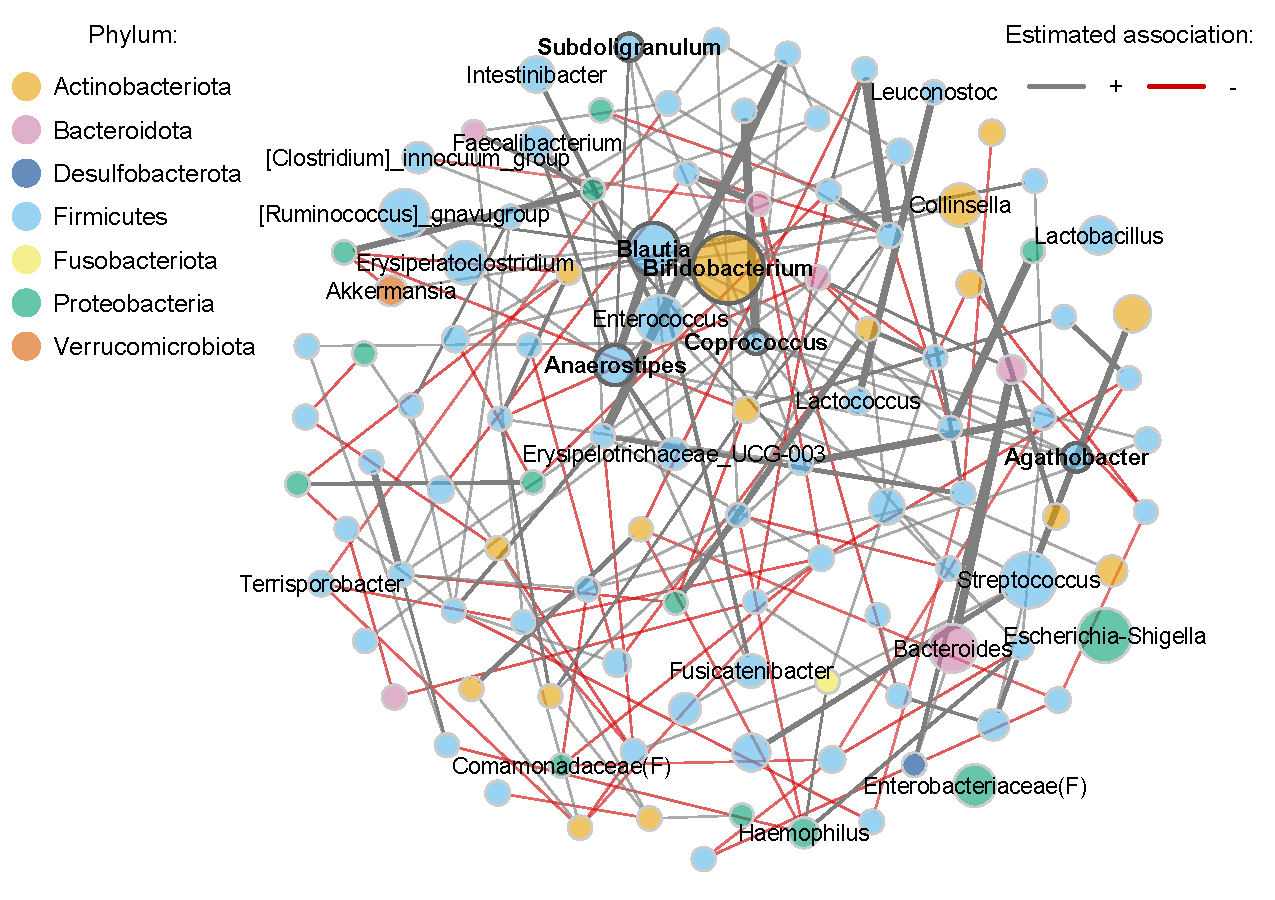
\includegraphics[width=\textwidth]{../ch07_application/figures/10_network_analysis/single_net_plot_spring_ownlay-1.pdf}
\caption{\textbf{SPRING association network with spring layout.} The network was estimated from the complete default data set using SPRING with the StARS settings described in Section~\ref{sec:7app:network:sensitivity}. Nodes represent genera and are colored according to phylum, while node sizes are proportional to the mean mCLR coordinate across samples. Gray and red edges indicate positive and negative estimated conditional associations, respectively. Node positions were determined by a force-directed layout based on the SPRING network itself. Labels identify genera highlighted in the preceding abundance, differential abundance, or differential distribution analyses, as well as selected highly connected genera.}
\label{fig:app:7app:net_single_spring}
\end{figure}

%====================================
\section{Network comparison}
\label{sec:app:7app:net_compare}
%====================================

\begin{figure}[H]
\centering
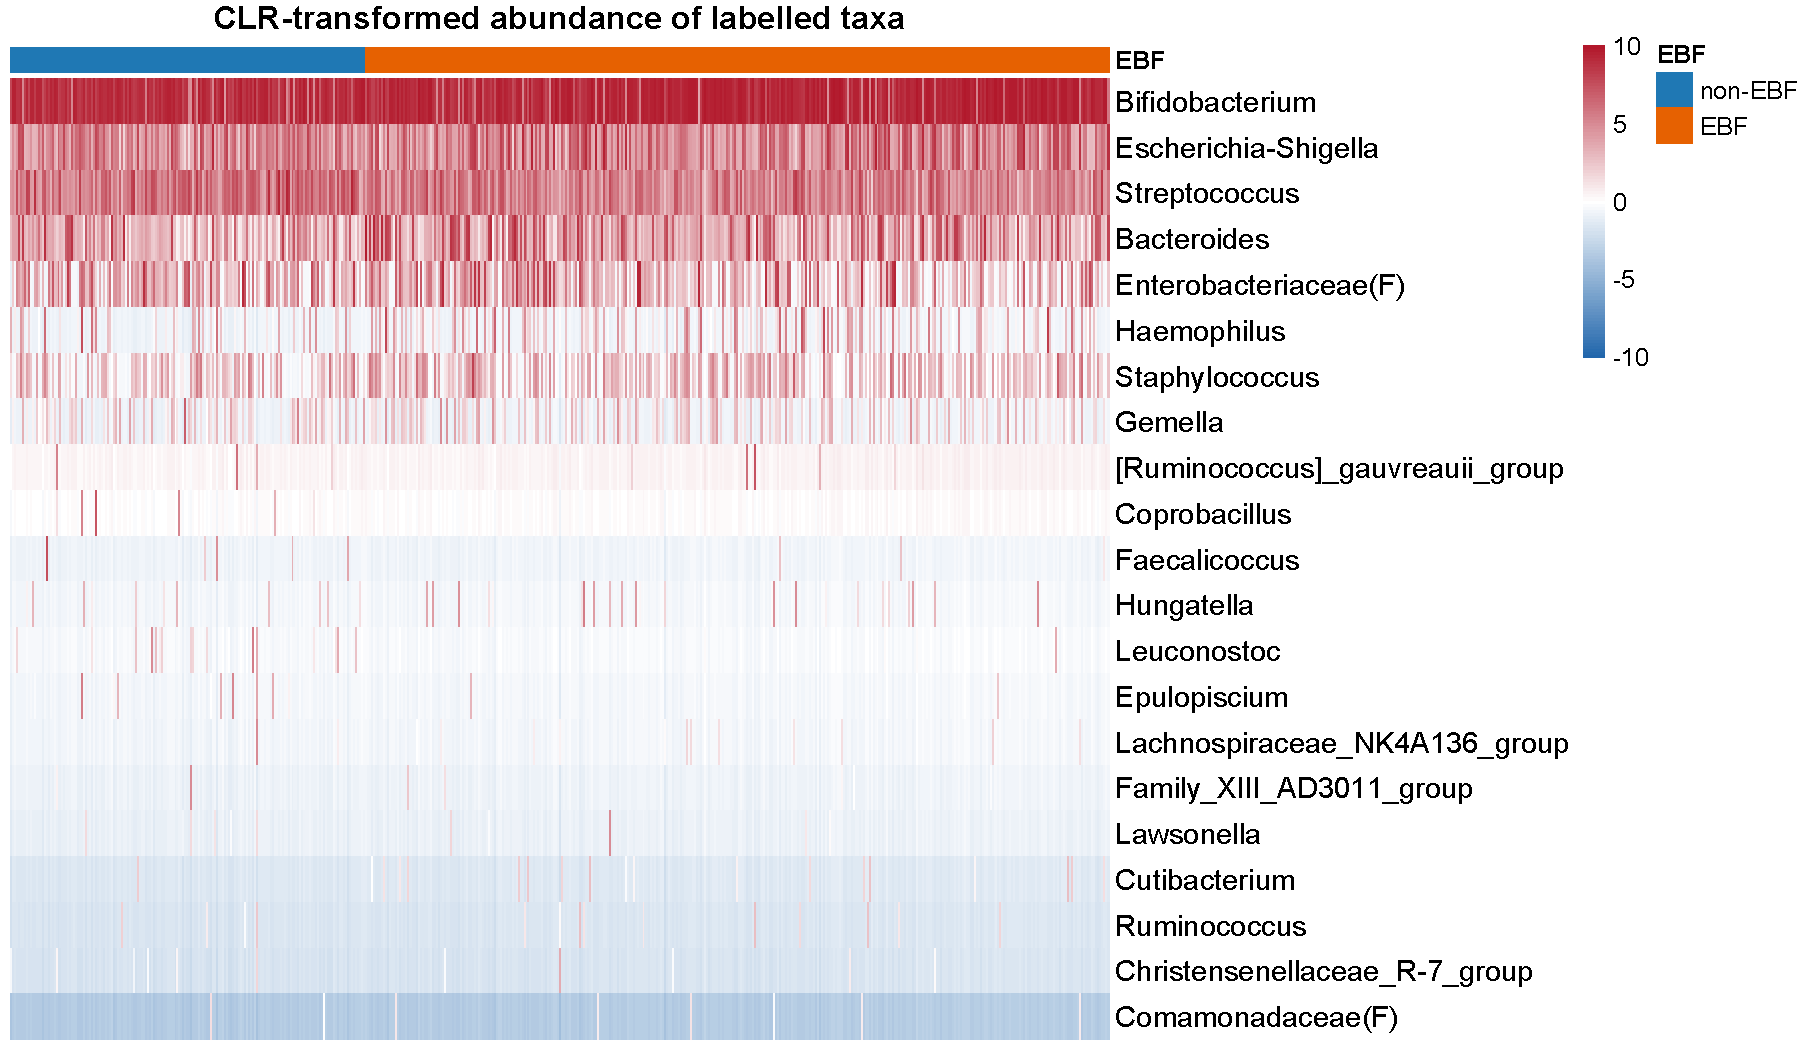
\includegraphics[width=\textwidth]{../ch07_application/figures/11_network_comparison/thesis_labelled_taxa_clr_heatmap-1.pdf}
\caption{\textbf{CLR-transformed abundances of selected genera.} The heatmap shows CLR coordinates after Bayesian-multiplicative replacement for the genera highlighted in Figure~\ref{fig:7app:network:ebf_network}. Columns represent samples and rows represent genera. Samples are ordered by EBF group. The transformed values form the fixed sample representation used for correlation-shrinkage network estimation in the differential network and differential association analyses.}
\label{fig:app:7app:net_compare_clr_heatmap}
\end{figure}

\begin{figure}[H]
\centering
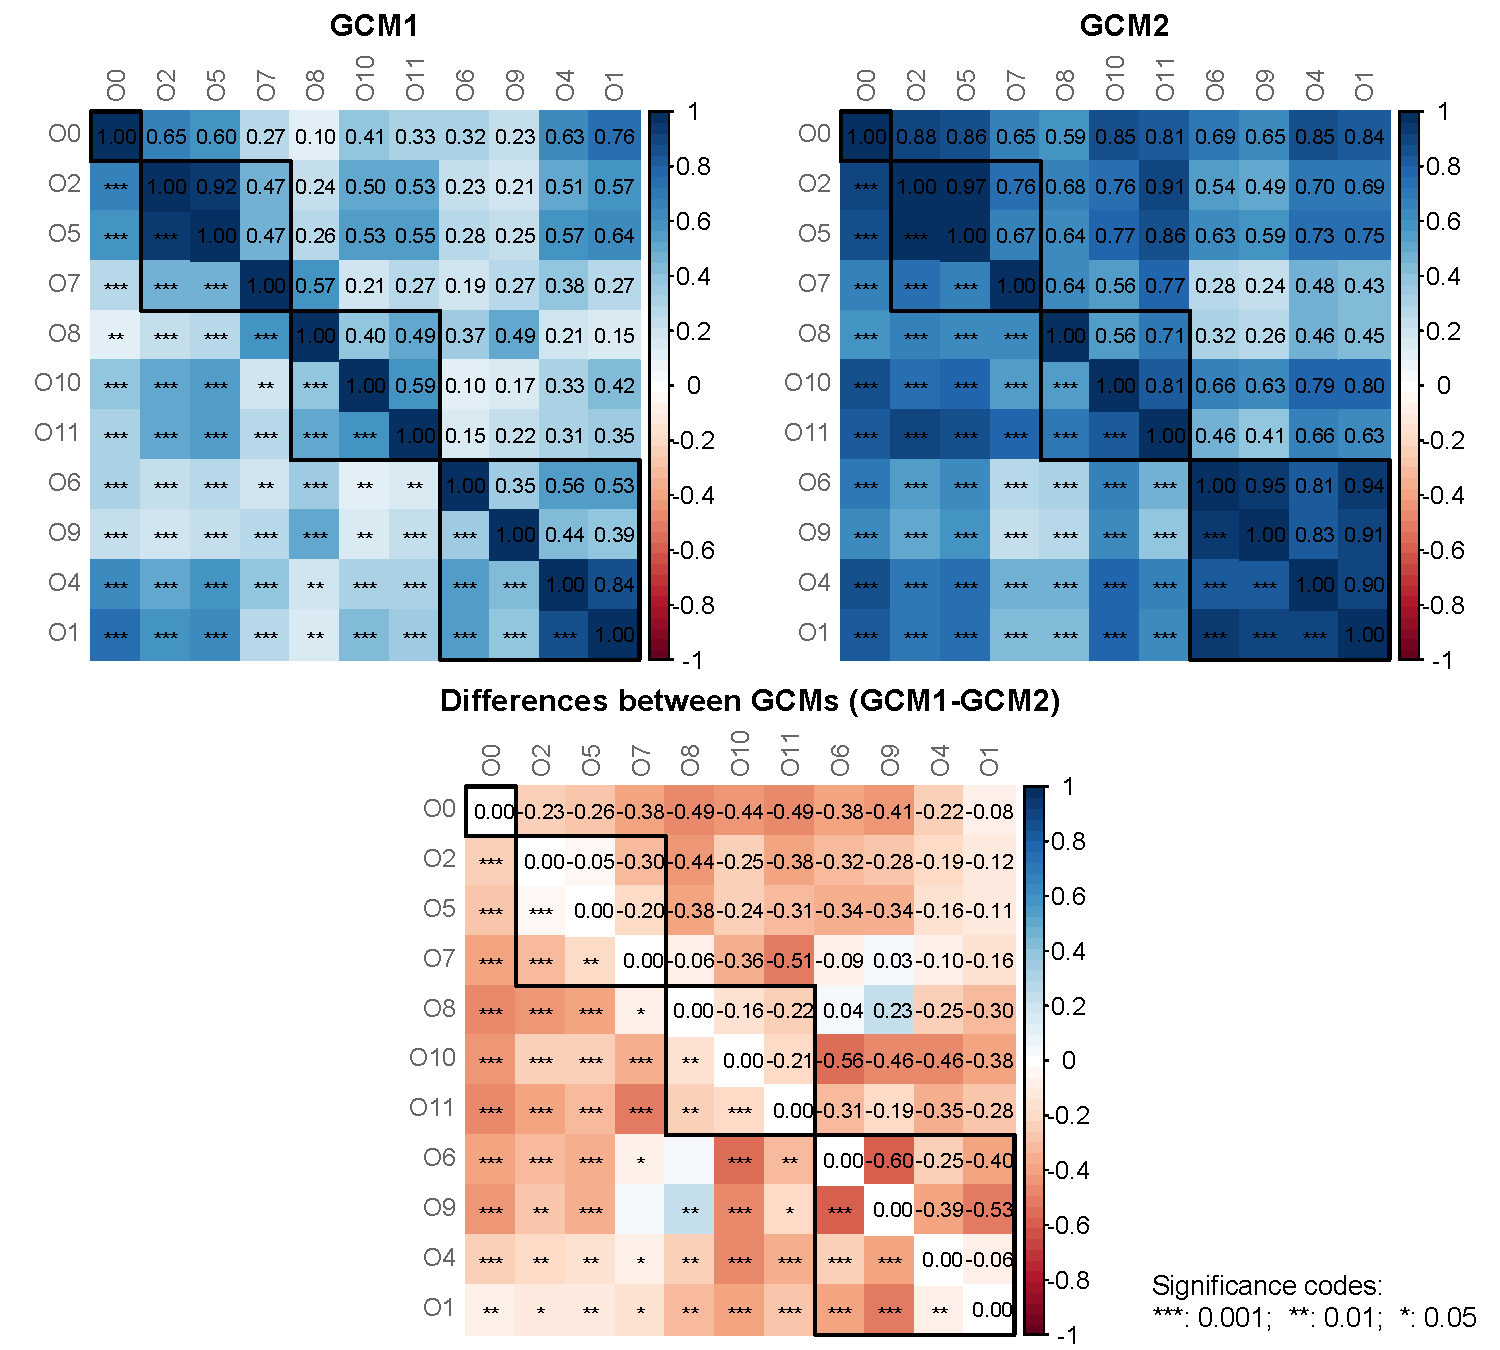
\includegraphics[width=\textwidth]{../ch07_application/figures/11_network_comparison/ebf_corshrink_bayesMult_gcm-1.pdf}
\caption{\textbf{Graphlet correlation matrices for the two EBF groups.} The upper panels show the graphlet correlation matrices (GCMs) of the correlation-shrinkage networks estimated after Bayesian-multiplicative replacement for children with EBF duration $=0$ and EBF duration $\geq 2$, respectively. Entries represent Spearman correlations between the non-redundant graphlet-orbit counts defined in Section~\ref{sec:5net:net_analysis:graphlets}. The lower panel displays the element-wise difference between the two matrices, computed as GCM$_{\mathrm{EBF}=0}$ minus GCM$_{\mathrm{EBF}\geq2}$. Asterisks indicate the significance level of the corresponding Fisher test.}
\label{fig:app:7app:net_compare_gcm}
\end{figure}
